 \documentclass{article}
\usepackage[utf8]{inputenc}
\usepackage{graphicx}

 \linespread{1.1}



\usepackage{tikz}
\usetikzlibrary{positioning}

\usepackage{amsmath,amssymb}
\usepackage{hyperref}
\usepackage{xcolor}
\usepackage{listings}
\usepackage{xcolor}
\usepackage{graphicx}
\graphicspath{{./images/}}
\usepackage{float}
\usepackage{natbib}
\bibliographystyle{abbrvnat}
\setcitestyle{authoryear,open={(},close={)}}
\raggedbottom

\definecolor{codegreen}{rgb}{0,0.6,0}
\definecolor{codegray}{rgb}{0.5,0.5,0.5}
\definecolor{codepurple}{rgb}{0.58,0,0.82}
\definecolor{backcolour}{rgb}{0.95,0.95,0.92}
\definecolor{myyellow}{rgb}{0.7,0.4,0}


\lstdefinestyle{mystyle}{
    backgroundcolor=\color{backcolour},   
    commentstyle=\color{codegreen},
    keywordstyle=\color{magenta},
    numberstyle=\tiny\color{codegray},
    stringstyle=\color{codepurple},
    basicstyle=\ttfamily\footnotesize,
    breakatwhitespace=false,         
    breaklines=true,                 
    captionpos=b,                    
    keepspaces=true,                 
    numbers=left,                    
    numbersep=5pt,                  
    showspaces=false,                
    showstringspaces=false,
    showtabs=false,                  
    tabsize=2
}

\lstset{style=mystyle}


\DeclareRobustCommand{\bbone}{\text{\usefont{U}{bbold}{m}{n}1}}

\DeclareMathOperator{\EX}{\mathbb{E}}% expected value






\title{Reasoning Agents Project}
\author{Cardia Francesca\\
        Coppa Federica\\
        Del Vecchio Andrea}
\date{July 2021}

\begin{document}



\maketitle

\section{Introduction}
The aim of this project consists in developing a non-Markovian agent able to solve a \textbf{navigation task with non markovian rewards} (using \textit{ Gym-Sapientino case environment}). The interesting aspect of the problem at hand is that the goal is characterized by a sequence of actions that a standard RL agent could not solve. For this reason we combined a RL agent with an automaton. Specifically, the algorithm we use for the agent is \textit{Proximal Policy Optimization} (PPO) and the automata are Deterministic Finite Automata (DFAs).

\section{Deterministic Finite Automata}
A Deterministic Finite Automaton (DFA) (as for instance \cite{dfa})
is a mathematical model that maps an input sequence to an output.  The result is that the computation is unique. A DFA can be exactly in one state at a given time and it makes the transition from one state to another state given some input and according to the transition function.\\
It is characterized by a tuple $\langle Q, \Sigma, \delta, q_o ,F \rangle$, where $Q$ is the set of states, $\Sigma$ is the set of symbols (alphabet), $\delta$  is the transition function $Q \times \Sigma \longrightarrow Q$ that takes as input a state and a symbol and returns a state, $q_o \in Q$ is the initial state and $F \subseteq Q$ is the set of final states (or accepting states).





\section{Proximal Policy Optimization}
Proximal Policy Optimization (PPO) is a family of policy gradient algorithms that became popular in recent years \cite{schulman2017proximal_PPO}. A policy gradient algorithm defines its objective in terms of the \textbf{gradient of the logarithm of the policy}. The policy, in this case, is a parametric probability distribution over the available actions in the current state.

\begin{equation}\label{eq:policyGradientObj}
\hat{g} = \EX[\nabla_{\theta}\log(\pi_{\theta}(a_{t}|s_{t}))A_{t}]
\end{equation}

PPO most common implementations represent \(\pi_{\theta}(a_{t}|s_{t)}\) with a (deep) neural network, which takes as input a state representation \(s_{t}\) and produces the value \(\pi_{\theta}\). \(\theta\) is the set of parameters of the neural network which get updated to maximize the policy gradient objective, usually by means of a stochastic gradient ascent algorithm.\\
To optimize the policy gradient objective [\ref{eq:policyGradientObj}], the algorithm should maximize not only the logarithmic term, which represents the contribution of the policy to the objective function, but also the \textbf{advantage term} \(A_{t}\) which can be interpreted as a measure of the benefits of taking that particular action \(a_{t}\) in the time step \(t\). \\
PPO original version defines the advantage function as:
\begin{equation}\label{eq:advantageDefinition}
A_{t}= \sum_{k=1}^{T}\gamma^{k}r_{t+k} \: - V_{\theta_{V}}(s_{t})
\end{equation}

\noindent
It is essentially a difference between the actual value of the action which is expressed in terms of the \textbf{expected discounted cumulative reward} where \(\gamma\) is the discount factor (first term in equation [\ref{eq:advantageDefinition}])

and a baseline estimate of state value \(V_{\theta_{V}}(s_{t})\) following that policy (the second term in the equation [\ref{eq:advantageDefinition}]). The baseline estimate is an estimation of the value of the cumulative discounted future reward given that action selection and following the current policy. It is a parametric function and, in deep reinforcement learning, is implemented as a neural network as well, called

%Ma come è trainata questa neural network (della baseline estimate)(??). Per minimizzare la LVF loss function.

\textbf{baseline network}, which takes as input the current state \(s_{t}\) and produces such estimate. The network is trained to minimize the a mean squared error loss between a \textit{target} state value (the real value of a state) and the estimated state value which is the output of the baseline network (see the \textit{value function term} in the equation [\ref{eq:completeObjective}]).\\ 
To clearly explain the meaning of the advantage function, it is convenient to study both the two cases in which \(A_{t}\) is greater or smaller than 0 respectively:
\begin{itemize}
\item \(A_{t}>0\): it means that the action has produced a (discounted, cumulative) reward which is better than the baseline estimate. For this reason, we address the execution of the action \(a_{t}\) as advantageous and we would like that the algorithm increases the probability of selecting the same action in the future (given the same state).
\item \(A_{t}<0\): it is the opposite case. The action is disadvantageous and we would like to decrease the probability of its selection in the future.
\end{itemize}
In order to avoid to produce excessively large updates of the policy parameters, which is a common problem of policy gradient algorithms, PPO substitutes the policy gradient objective [\ref{eq:policyGradientObj}] with the \textbf{clipped surrogate} objective function defined as:

\begin{equation}\label{eq:clippedSurrogateObjective}
L^{CLIP}(\theta) = \hat{\EX}[\min(r_{t}(\theta)A_{t}, clip(r_{t}(\theta),1-\epsilon,1+\epsilon)A_{t}]
\end{equation}

\begin{figure}
    \centering
    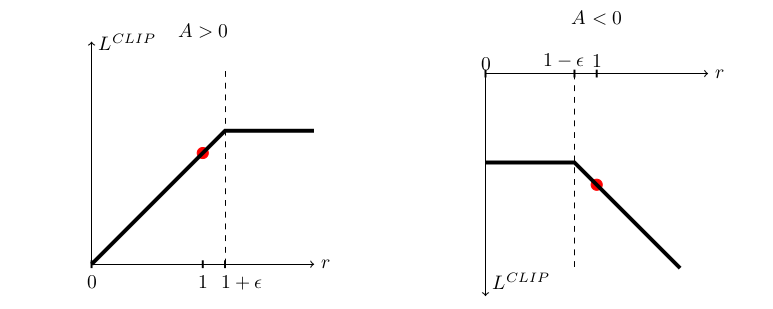
\includegraphics[width = \textwidth]{images/L_clip_image.png}
    \caption{Figure representing the effect of the clipping operation on the surrogate objective function. The figure is taken from the paper \cite{schulman2017proximal_PPO}.}
    \label{fig:ClippingObjective}
\end{figure}
%Inserire da appunti if the action was good...If the action was bad... nella caption se necessario.

Where the expected value, in this case, is taken as the empirical average of a batch of samples.\\
The variable \(r_{t}(\theta)\) is defined as
\begin{equation}\label{eq:ratioR}
r_{t}(\theta) = \frac{\pi_{\theta}(a_{t}|s_{t})}{\pi_{\theta_{old}}(a_{t}|s_{t})}
\end{equation}
and represents the probability ratio between the currently considered policy and the older policy, which is the policy of the agent before the last update. \\
If \(r_{t}(\theta) > 1\), the action \(a_{t}\) is more likely to be selected in the current policy than in the older policy, and  we have \(r_{t}(\theta) \in  [0,1)\) in the opposite scenario.\\
The clipped surrogate objective forces the algorithm to perform conservative updates if the advantage estimate \(A_{t}\) become too large in magnitude. An update is said to be conservative if the updated policy is not \textit{"too far away"} (in terms of the Kullback-Leibler divergence 

\footnote{The Kullback-Leibler divergence measures the difference between two probability distributions and is defined as \(KB(P||Q = \sum_{i}P(i) \log_{2}\left(\frac{P(i)}{Q(i)})\right)\) where \(P\) and \(Q\) are two discrete probability distributions. }) 

 from the older policy.\\
\(\epsilon\) is an hyperparameter of the algorithm and must be defined before instantiating the agent. The authors of the paper suggest using \(\epsilon= 0.2\) but other choices are also possible.\\

The most common implementation of the PPO   objective function is composed by three terms \cite{schulman2017proximal_PPO}.

\begin{equation}\label{eq:completeObjective}
L^{CLIP+VF+S}(\theta) = \hat{\EX}[L^{CLIP}(\theta) + c_{1}L^{VF}(\theta)+c_{2}S[\pi_{\theta}](s_{t})]
\end{equation}

\noindent
The first is the clipped surrogate objective function. \\
The second term is a \textit{squared loss} term associated to the output of the baseline network. We call this term \textit{value function term} for simplicity.
\begin{equation}
L^{VF}= (V_{\theta}(s_{t})- V_{t}^{targ})^{2}
\end{equation}
The combination of the clipped surrogate objective term and of the value function term allows the algorithm to share parameters between the policy and the baseline networks. \(c_{3}\) is the coefficient of the \textbf{entropy bonus} and ensures sufficient exploration \cite{schulman2017proximal_PPO}. 





\section { Markov Decision Process}
The general setting of Reinforcement Learning is the following:\\

\includegraphics[scale=0.83]{images/agent.png}
\noindent\\
The agent at the state $S_t$ executes an action $A_t$ and receives from the environment an associated reward.
Most of RL algorithms assume that the environment can be modeled as MDP.\\
Markov Decision Processes (MDPs) are a central model for sequential making under uncertainty.
A Markov Decision Process (MDP) is a tuple $\langle S,A,T,R,\gamma \rangle$, where $S$ are the states, $A$ are the actions called action space,  $T$ the transition function $T: S \times A \longrightarrow Prob(S)$ that returns for every state $s$ and action $a$ a distribution over the next state ($T(s,a,s')=P(s'|s,a)$). $R$ represents the reward function $R: S \times A \longrightarrow \mathbb{R}$ that specifies the real valued reward received by the agent when applying action $a$  in state $s$ ($R(s,a,s')$ $\in$ $\mathbb{R}$)  and $\gamma$ represents the discount factor.\\\\
\begin{figure}[h!]
    \centering
    \includegraphics[scale=0.9] {images/mdp.png}
    \caption{MDP example}
    \label{fig:mdp}
\end{figure}

\noindent 
The next state $s_{t+1}$ is not dependent from $s_{t-1}$, and consequently is not dependent from the history.
In fact looking at figure [\ref{fig:mdp}] we can observe that if we remove $s_t$ the graph becomes disconnected.\\
Then the following properties hold:\\\\
\begin{equation}
\label{one}
s_{t+1}  \perp  s_0, . . . , s_{t-1} | s_t \quad \forall t
\end{equation}

\begin{equation}
\label{two}
r_{t+1} \perp  s_0, . . . , s_{t-1}| s_t \quad \forall t\\
\end{equation}

\noindent


\noindent
So the next state is not dependent from the history if the current state $s_t$ is given. The same holds for rewards.
A solution to an MDP is called \textit{policy}, and it assigns an action to each state, possibly conditioned on past states and actions.
Every MDP has an \textit{optimal policy}, which maximizes the expected sum of rewards for every starting state $s \in S$.


\section{Non Markovian Rewards Decision Processes}
A Non Markovian  Decision Process is a stochastic process that does not exhibit the Markov properties [\ref{one}],
[\ref{two}] (generalized as  memoryless property).
A Non Markovian Reward Decision Process (NMRDPs) is a tuple $M= \langle S, A, T, R, \gamma \rangle$, where S,A, T, $\gamma$ are equivalent to MDPs case, while R is redefined as $\bar{R}:(S\times A)^* \longrightarrow \mathbb{R}$.\\
Now  the reward  is a real valued function over finite state-action sequences (according to a specific history).


\paragraph{Temporal rewards specifications}
\noindent\\\\
In these cases, we have a set of episodes (traces $\pi$), in fact the temporal logics needs to talk about set of temporal traces.
The concept is the following: we have a temporal formula $\phi$ and we can observe all traces that satisfy this formula.
The steps are the following:
\begin{itemize}
\item Define an alphabet of propositional symbols (fluents)
\item Define labelling function $f_F:S\times A \longrightarrow 2^F$
\end{itemize}
\noindent
These definitions induce a trace $\pi$ of propositional interpretations:\\ $ (S\times A)^*\xrightarrow{f_F}  (2^F)^*$.\\
In order to define the non-markovian reward, we firstly define a set of formulas with associated reward $\{(\phi_i,r_i)\}_{i=1} ^m$.
Then  the non-markovian reward is :\\

\begin{figure}[h]
   \centering
\includegraphics[scale=0.65]{images/NMreward.png}\\
\end{figure}

\noindent
in particular, if episode (trace $\pi$) satisfies formula $\phi$ it generates a reward.


\paragraph{Rewarding with automata}\\
\noindent\\\\
Any LTLf/LDLf formula $\phi$ can be converted to DFA that recognizes the same traces ($A_\phi=\langle Q_\phi, q_{o\phi},\Sigma, F_\phi\rangle$). Practically we can translate Non-Markovian Rewards Decision Process into a MDP with state space:
$S'= S \times Q_{\phi(1)}\times .... \times Q_{\phi(m)}$\\
\noindent
This is a cross product, where $S$ is the set of states and $Q_{\phi(i)}$ (with $i=1,..,m$) are the automaton states.



\section{Gym-Sapientino}
This is a new RL discrete environment that respects the gym interface \cite{Gym-Sapientino}.\\
It is characterized by a map which contains a sequence of colors (represented by colored cells). \\
The agent can move in the map executing actions that have continuous effects on the state, moreover also the observations received from the environment are continuous. The observations that are continuous on the state, are characterized by the \textit{position}, the \textit{linear velocity} and  the \textit{angular velocity}. \\
In fact the agent executes an action, the environment returns an associated reward and an observation on the state and on automaton state.

\subsection{Temporal Goal on Gym-Sapientino}

The non markovian agent moves in the map executing a non markovian task (the ordered visit of a sequence of colors). 
In particular it should reach
temporal goals, described properly by a specific sequence of colors. When the agent reach a temporal goal it receives a reward from the environment, and more frequently it earns rewards more it will be prodded to learn.\\
This environment allows to work with four different colors ( and consequently with a temporal goal characterized by four components):\\
{\color{myyellow}\textbf{yellow}}, {\color {blue} \textbf{blue}}, {\color{codegreen} \textbf{green}}, {\color{red} \textbf{red}}.

\noindent
%Gym-Sapientino uses LYDIA in order to convert temporal goals into automata.
It is possible to specify which colors are included in the temporal goal formulas $\phi$, and consequently in the related automaton $A_\phi$ (which is provided by the environment). 
In the automaton the states related to the colors are specified through numbered codification. Moreover there is a particular failure state, denoted previously as \textit{SINK}, that we have converted into numbered codification using 2 to indicate it. Then, if we consider a map characterized by two colors, for instance \textit{blue} and \textit{green}, the related automaton will be composed by four numbered states as showed in \ref{fig:stati} :

\vspace{2em}
\begin{figure}[H]
\centering
\includegraphics[width=0.85\linewidth]{stati}
\caption{Representation of the problem at hand in term of automata}
\label{fig:stati}
\end{figure}

\noindent
Notice that \texttt{0} is the initial state and \texttt{3} is the accepting state.
In this case the agent can reach the temporal goal visiting the following sequence: \texttt{0,1,3}. In order to control the correct achievement of the temporal goal, we have also interfaced with the following problem:\\
in Gym-Sapientino environment the agent can execute some actions signaled by five particular  strings: \texttt{LEFT}, \texttt{RIGHT}, \texttt{FORWARD}, \texttt{NULL}, \texttt{BEEP}. The first,the second and the third need to indicate in which direction the agent is moving, the fourth needs to signal that the agent is not moving and the last needs to signal that the agent is visiting a certain state.
The problem rises when the agent enters in the same state twice consecutively, and this implies a double \texttt{BEEP} visualization. In our work we have controlled this problem, avoiding that the current state reached by the agent was equal to the previous reached state. In this case we impose that the temporal goal is satisfied only when the sequence of states does not include equal states. For instance in the previous example with two colors ( blue and green):\\
the temporal goal is reached when is visited this sequence \texttt{0,1,3} and not \texttt{0,1,1,3} or \texttt{0,1,3,3}.




%\section{Reward shaping}
%Most of the techniques in Reinforcement Learning (RL) assumes that the learning starts from a blank slate and improves only by means of trial and error. This learning approach takes a huge amount of trials and as a direct consequence it implies that the time required is a lot. This is why we talk about \textbf{reward shaping} \citep{rf}. This method is useful to incorporate domain knowledge in the RL agents. In reward shaping, the domain knowledge is represented as a supplementary reward that allows the RL agent to learn more efficiently.
%A Deterministic Finite Automaton (DFA) \citep{dfa} is a mathematical model that maps an input sequence to an output. The result is that the computation is unique. A DFA can be exactly in one state at a given time and it makes the transition from one state to another state given some input and according to the transition function.\\
%In our code the \textbf{Reward shaping} has been implemented and applied as showed in \ref{fig:reward shaping}, where according to \ref{fig:stati} the agent received a great reward of 500 when reaching the right state, otherwise in case of \textit{SINK\_ID} the reward is -500.

%\vspace{2em}
%\begin{figure}[H]
%\centering
%\includegraphics[width=\linewidth]{rs}
%\caption{Reward shaping}
%\label{fig:reward shaping}
%\end{figure}

\section{The non markovian agent}
Since we have to solve a non markovian problem, the agent must take into account past experience in order to select the optimal action. In this case, the agent is said to be \textbf{non markovian}.
To build a non markovian agent, we might start considering the problem of visiting the color sequence as a composition of a number of smaller sub-problems: for example, given the goal \{\color{blue} blue \color{black}, \color{red} red \color{black}, \color{green} green \color{black} \}, we extract three sub-problems which are purely markovian:
\begin{enumerate}
    \item Visit the \color{blue} blue \color{black} color.
    \item \textbf{Then} visit the \color{red} red \color{black} color.
    \item \textbf{Finally} visit the \color{green} green \color{black} color.
\end{enumerate}
In this way we end up reducing the original, non markovian problem, to a set of markovian problems which we can solve \textbf{sequentially} using SOA methods.\\
%Spiegare perchè i problemi sono markovian (?).


Moreover, this approach completely cuts out the issue of keeping track of past state, action and reward traces.\\
With this in mind, we can build 3

%Controllare dal punto di vista teorico la parte scritta in grassetto per sicurezza.
\footnote{In general, the more colors are involved in the goal sequence, the higher is the number of markovian agents we have to train. In the case of a sequence of the type \{\color{blue}blue\color{black},\color{green}green\color{black},\color{red}red\color{red},\color{blue}blue\color{black}\} there is no need to build an additional agent for the last blue color in the sequence, as we already have at our disposal an agent which can reach the blue color (the first one). \textbf{This happens because agents are associated to colors and not to sequence elements}. \\
Be aware that, theoretically, the proposed implementation supports sequences of arbitrary size.} 

separate markovian agents and train them to reach the corresponding colored tile in the map (figure [\ref{fig:mapTwoColors}], [\ref{fig:mapThreeColors}]). \\


\begin{figure}
    \centering
    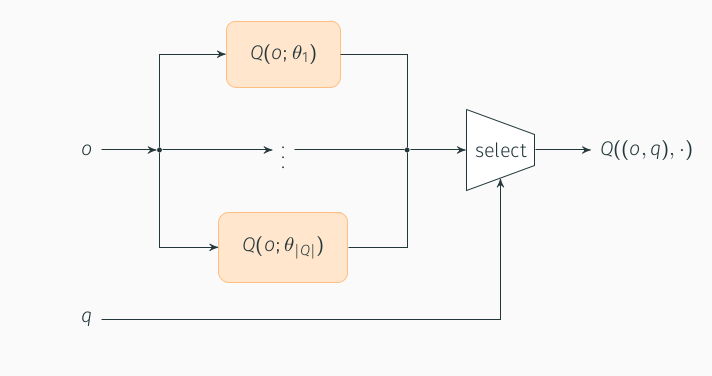
\includegraphics[width=\textwidth]{images/baseline_implementation_schema.png}
    \caption{Baseline implementation for the non markovian policy network. It takes as input both an observation \(o\), the state vector in our problem, and the state of the goal DFA \(q\). Then, according to the state of the automaton, the agents selects one of the \(|Q|\) \textit{separate experts} (the markovian agents we have discussed so far) for the action selection. This image is taken from the slides of Roberto Cipollone for the Reasoning Agent course held in Sapienza in 2020/2021.}
    \label{fig:baselineSchema}
\end{figure}



However, at any given time, only one markovian agent can select an action to execute (figure [\ref{fig:baselineSchema}]). \\
The action selection is constrained by the goal formulation. In fact, we consider the gym Sapientino task to be solved if and only if the non markovian agent visits the colors \textbf{in the order in which they appear in the temporal goal formula}. In fact, if the agent visits the colors in the wrong order (for example \{\textit{blue},\textit{green}, \textit{red}\} instead of \{\textit{blue}, \textit{red}, \textit{green}\}) 

%Sinks (?)
the automaton goes in the \textit{sink} state and episode terminates with a failure.\\

\noindent
To reach the goal,then, the agent must be aware of which color in the goal sequence it has already visited and which color is the next one in the sequence. Such an information may be inferred by inspecting the states of the goal DFA. (see the example in figure [\ref{fig:stati}].
%(riferimento alle figure dei goal DFA)
%In fact, once the agent correctly visits a portion of the formula (\color{blue} blue \color{black} for the problem considered), the DFA changes the state. If the resulting state is accepting, it means that the agent has visited the whole formula; otherwise there are still some colors to visit.\\%
Luckily the environment allows the agent to keep track of the automaton states. 
Therefore, in order to visit the goal, it is sufficient to select, from time to time, the "correct" markovian agent depending on the automaton state (see figure [\ref{fig:nonMarkovianNetwork}] for a  graphical explanation) .
\noindent
In the section below, we present our solution for the expert selection in the context of a popular deep reinforcement learning open source framework. The approach focuses on efficiency and network parameter sharing and is based on parallel computation and automatic differentiation.\\



%The code below is based on the tutorial https://latexdraw.com/drawing-neural-networks-in-tikz-short-guide/

%Define the number of input neurons.
\newcommand{\inputnum}{7}

%Define the number of hidden neurons.
\newcommand{\hiddennum}{9}

%Define the number of output neurons.
\newcommand{\outputnum}{5}


%Define the position on the x-axis of the first hidden layer neurons.
\newcommand{\firstHiddenNeuronsPosition}{3.0}


%Define the position on the x-axis of the second hidden layer neurons.
\newcommand{\secondHiddenNeuronsPosition}{6.0}


%Define the position on the x-axis of the output layer neurons.
\newcommand{\outputNeuronsPosition}{9.0}

%Define the position of the oneHotEncoding for the first hidden layer.
\newcommand{\oneHotEncodingFirstHidden}{3.5}


%Define the position of the oneHotEncoding for the second hidden layer.
\newcommand{\oneHotEncodingSecondHidden}{6.5}



%Define the number of output neurons.


\begin{figure}

\begin{tikzpicture}[x=1.5cm, y=1.5cm, >=stealth]


%Input neurons
\foreach \i in {1,...,\inputnum}
{
    \node[circle, 
		minimum size = 6mm,
		fill=orange!30] (Input-\i) at (0,-\i) {};
}

%First hidden layer.
\foreach \i in {1,2,3}
{
    \node[circle, 
		minimum size = 6mm,
		fill=blue!100,
		yshift =(\hiddennum-\inputnum)*5mm] (Hidden-\i) at (\firstHiddenNeuronsPosition,-\i) {};
}

\foreach \i in {4,5,6}
{
    \node[circle, 
		minimum size = 6mm,
		fill=red!100,
			yshift =(\hiddennum-\inputnum)*5mm] (Hidden-\i) at (\firstHiddenNeuronsPosition,-\i) {};
}

\foreach \i in {7,8,9}
{
    \node[circle, 
		minimum size = 6mm,
		fill=green!100,
			yshift =(\hiddennum-\inputnum)*5mm] (Hidden-\i) at (\firstHiddenNeuronsPosition,-\i) {};
}


%One hot encoding for the first hidden layer
\foreach \i in {1,2,3}
{
 \node[circle, 
		minimum size = 6mm,
		fill=magenta!100,
			yshift =(\hiddennum-\inputnum)*5mm] (OneHotHidden1-\i) at (\oneHotEncodingFirstHidden,-\i) {1};

}


\foreach \i in {4,5,6,...,9}
{
 \node[circle, 
		minimum size = 6mm,
		fill=magenta!100,
			yshift =(\hiddennum-\inputnum)*5mm] (OneHotHidden1-\i) at (\oneHotEncodingFirstHidden,-\i) {0};

}



%Second hidden layer.
\foreach \i in {1,2,3}
{
    \node[circle, 
		minimum size = 6mm,
		fill=blue!100,
			yshift =(\hiddennum-\inputnum)*5mm] (Hidden2-\i) at (\secondHiddenNeuronsPosition,-\i) {};
}

\foreach \i in {4,5,6}
{
    \node[circle, 
		minimum size = 6mm,
		fill=red!100,
			yshift =(\hiddennum-\inputnum)*5mm] (Hidden2-\i) at (\secondHiddenNeuronsPosition,-\i) {};
}

\foreach \i in {7,8,9}
{
    \node[circle, 
		minimum size = 6mm,
		fill=green!100,
			yshift =(\hiddennum-\inputnum)*5mm] (Hidden2-\i) at (\secondHiddenNeuronsPosition,-\i) {};
}



%One hot encoding for the second hidden layer
\foreach \i in {1,2,3}
{
    \node[circle, 
		minimum size = 6mm,
		fill=magenta!100,
			yshift =(\hiddennum-\inputnum)*5mm] (OneHotHidden2-\i) at (\oneHotEncodingSecondHidden,-\i) {1};
}
\foreach \i in {4,5,6,...,9}
{
    \node[circle, 
		minimum size = 6mm,
		fill=magenta!100,
			yshift =(\hiddennum-\inputnum)*5mm] (OneHotHidden2-\i) at (\oneHotEncodingSecondHidden,-\i) {0};
}

%Output layer.
\foreach \i in {1,...,\outputnum}
{
    \node[circle, 
		minimum size = 6mm,
		fill=orange!30,
		yshift = (\outputnum-\inputnum)*5mm
		] (Output-\i) at (\outputNeuronsPosition,-\i) {};
}


% Connect neurons In-Hidden
\foreach \i in {1,...,\inputnum}
{
	\foreach \j in {1,...,\hiddennum}
	{
		\draw[->, shorten >=1pt] (Input-\i) -- (Hidden-\j);	
	}
}

% Connect neurons Hidden-Hidden2
\foreach \i in {1,...,\hiddennum}
{
	\foreach \j in {1,...,\hiddennum}
	{
		\draw[->, shorten >=1pt] (OneHotHidden1-\i) -- (Hidden2-\j);
	}
}


% Connect neurons Hidden2-output
\foreach \i in {1,...,\hiddennum}
{
	\foreach \j in {1,...,\outputnum}
	{
		\draw[->, shorten >=1pt] (OneHotHidden2-\i) -- (Output-\j);
	}
}








\end{tikzpicture}
\caption{This sketch represents the non markovian policy network scheme implemented as a two hidden layer fully connected neural neural network. The architecture in the figure may employed in solving the problem of visiting a sequence of three colors  (\color{blue} blue \color{black}, \color{red} red \color{black} and \color{green} green \color{black}). In \color{magenta} magenta\color{black}, we represent the automaton state binary vector as described in the section [\ref{sec:ImplementationDetails}]. The \color{blue} blue \color{black} neurons represent the policy network of the markovian agent that is trained to reach the \color{blue} blue \color{black} colored tile in the map; the same holds for the \color{red} red \color{black} and the \color{green} green \color{black} neurons.}
\label{fig:nonMarkovianNetwork}
\end{figure}


\section{Implementation Details}\label{sec:ImplementationDetails}

For the agent implementation we have used Tensorforce \footnote{ The latest version of Tensorforce documentation can be found at \url{https://tensorforce.readthedocs.io/en/latest/}}, an open source library for deep reinforcement learning based on Tensorflow and Keras. Tensorforce supports a variety of deep RL agents like DQN, PPO, DDPG and features the most common neural network architectures (dense, recurrent, convolutional, attention based) for policy network implementation.\\
Due to its ease of use and its great effectiveness, Tensorforce is one of the most frequently used frameworks for reinforcement learning experiments. However, as far as we know, the latest version of the library (Tensorforce 0.6.4) does not support non markovian agents implementation by default. Therefore, for the purpose of our project, we must manipulate the Tensorforce agent policy networks and adapt them to a non markovian framework.\\

\subsection{Proposed network implementation}
In this work, we propose a non markovian agent implementation inspired from [\ref{fig:baselineSchema}] which employs a single policy network for action selection. The architecture is divided in \textit{chunks} (or portions), each one assigned to a different markovian agent (or color) as described in the figure \ref{fig:nonMarkovianNetwork}.
We make each chunk of the same size and associate it to a different color in the goal sequence. The chunks so created


\footnote{Keep in mind that, in our project, we are assuming, for simplicity, that all the colors in the goal sequence are different. In other words no color repetition is allowed. Of course, this does not limit the applicability of our solution as discussed in the conclusion paragraph.} 

act as \textbf{policy network} for the markovian agents (the \textit{separate "experts"} described in figure [\ref{fig:baselineSchema}]). \\
To better explain how the proposed non markovian policy network implementation works, we include a brief textual description of the training loop algorithm of the agent: \\
for each step in a given episode, we sample the environment state, a seven elements vector, and the state of the automaton, an integer number. Afterwards, we create a binary \textit{encoding} of the automaton state which is built as follows:


%Fare disegnino del vettore che si costruisce (?)

\begin{enumerate}
    \item Instantiate a vector filled with zeros of size \(H * N\) where \(N\) is the number of automaton states and \(H\) is the size of each \textit{chunk} of the policy network.
    \item Divide the encoded state vector into equally sized sub-portions. Each portion will have a size of \(H\). The encoded state vector portions and the non markovian policy network \textit{chunks} described in the previous point must have the same size.
    \item Assign the sub-portions to a different automaton state.
    \item Fill the part corresponding to the \textbf{current automaton state} with \textit{ones} and leave the rest with \textit{zeros}.
    \item Multiply the binary vector to the output of each dense layer to \textbf{select}, from time to time, the \textit{chunk} of the network of interest (a subset of the neurons of the dense layer).
    \
\end{enumerate}
In this way we are able to select the chunks of the non markovian policy network which contribute to the action selection. In fact, the hidden layer neurons which are multiplied to 1 elements in the binary vector are kept in the forward pass and determines the action the policy network selects in the current state.\\ 
On the other hand, the neurons of the network multiplied by the zeros in the binary vector do not contribute to the action selection (they are \textit{"zeroed"} ) and simply \textbf{get discarded}.\\
Using this strategy, we are able to select all the network sub portions which correspond to the expert we would like to consider at any given time, discarding all the network chunks that correspond to the other experts (figure [\ref{fig:nonMarkovianNetwork}]).\\
In figure [\ref{fig:nonMarkovianNetwork}] we show a graphical example of a forward pass in the non markovian policy network. 
The input layer receives as input the 7 dimensional state vector returned by gym Sapientino environment at each iteration, while the two hidden layers are subdivided into three parts each one corresponding to a different color. The correct network sub-portion is selected by multiplying the binary vector, which is built according to the algorithm sketched above, to the output of each hidden layer. In this figure we sketch an example of execution in which we select the first three neurons only from the two hidden layers (the binary vector contains 1 in the first three elements and 0 in all the other elements). \footnote{This may happen, for example, if the goal sequence is G = \{\color{blue} blue \color{black}, \color{red} red \color{black},\color{green} green \color{black}\} and the agent has to visit the first color in the sequence.}
In the example, they correspond to the network sub-portion associated to the markovian agent which is learning (or has learnt yet) to visit the blue colored tile and so, this means that 
%Sciogliere la frase sotto...
the agent action selection focuses on reaching the blue color in the environment.\\
Below we give a more detailed description of the Tensorforce implementation of our non markovian policy network, commenting and motivating the role of each component in the overall architecture.







\subsection{Network Description}
\label{network}
We have implemented a custom network in the following way (figure [\ref{fig:nonMarkovianNetwork}]):\\
\begin{lstlisting}
network=dict(type = 'custom', 

    layers= [
    
    dict(type = 'retrieve',tensors= ['gymtpl0']),
    dict(type = 'linear_normalization'),
    
    dict(type='dense', bias = True,activation ='tanh',size=AUTOMATON_STATE_ENCODING_SIZE),
    
    dict(type= 'register',tensor = 'gymtpl0-dense1'),
    
    #Perform the product between the one hot encoding of the automaton and the output of the dense layer.
    dict(type = 'retrieve',tensors=['gymtpl0-dense1','gymtpl1'], aggregation = 'product'),
    
    dict(type='dense', bias = True,activation ='tanh',size=AUTOMATON_STATE_ENCODING_SIZE),
    
    dict(type= 'register',tensor = 'gymtpl0-dense2'), 
    
    dict(type = 'retrieve',tensors=['gymtpl0-dense2','gymtpl1'], aggregation = 'product'),
    
    dict(type='register',tensor = 'gymtpl0-embeddings'),],)
\end{lstlisting}

\noindent
This network is characterized by:\\
\begin{itemize}
    \item \textbf{Retrieve layers}: they are useful when defining more complex network architectures which do not follow the sequential layer-stack pattern, for instance when there are multiple inputs. It allows to aggregate multiple inputs  through concatenation, product,sum operations ( in our case we have used the product). 
    \item \textbf{Linear normalization layer}:  which scales and shifts the input to [-2.0, 2.0], for bounded states with min/max\_value. 
    \item \textbf{Register layers}: they are an other type of retrieval layers useful for complex networks and for multiple inputs.
    \item \textbf{Dense layers}: they are Dense fully-connected layers.
\end{itemize}

\subsection{Reward shaping}\label{sec:rewardShaping}
Most of the techniques in Reinforcement Learning (RL) assumes that the learning starts from a blank slate and improves only by means of trial and error. This learning approach takes a huge amount of trials which implies that the this method is a also very time consuming. This is why we talk about \textbf{reward shaping} \citep{rf}. This method is useful to incorporate domain knowledge in the RL agents. In reward shaping, the domain knowledge is represented as a supplementary reward that allows the RL agent to learn more efficiently.
%A Deterministic Finite Automaton (DFA) \citep{dfa} is a mathematical model that maps an input sequence to an output. The result is that the computation is unique. A DFA can be exactly in one state at a given time and it makes the transition from one state to another state given some input and according to the transition function.\\
In our code the \textbf{Reward shaping} has been implemented and applied as showed in \ref{fig:reward shaping}, where according to \ref{fig:stati} the agent received a great reward of 500 when reaching the right state, otherwise in case of \textit{SINK\_ID} the reward is -500.\\
In particular in our case the reward shaping technique is useful because the reward is positive and scattered. Moreover, we can monitor when the agent is approaching to the goal, in fact the path in the automaton is "obligated", so this is a good reason to reward the agent inciting to proceed.

\vspace{2em}
\begin{figure}[H]
\centering
\includegraphics[width=0.8\linewidth]{rs}
\caption{Reward shaping for two colors case; this mechanism can be extended also to three colors case.}
\label{fig:reward shaping}
\end{figure}




\section{Experimental environment}


In the following sections we discuss some experiment results on different gym Sapientino maps for a number temporal goals. \\
All the experiments we discuss are run on local machines with no GPUs equipped. This is possible as the network size is relatively small  . All the agents have been trained for a small number of episodes. 
The two color agents trained for 1000 episodes, whereas the three color agents trained for 2000 episodes. %We used the hyperparameter configuration which is reported in table [\ref{tab:easyMapAgentTable}] for all the experiments.

%TODO: inserire parametri utilizzati per gym sapientino (angular velocity, linear velocity ertc...)


\section{Trials}
We have done progressive trials in order to arrive to the situation in which the agent can reach a temporal goal characterized by three colors.
We have performed the training using CPU and we have collected the plots using \textbf{Tensorboard}.\\
In particular we focus the attention on the following plots:
\begin{itemize}
    \item \textbf{agent/cond/episode-length}: the mean length of each episode in the environment for all agents.
    Notice that the \textbf{x-axis} registers the number of episodes, while the \textbf{y-axis} the mean length of each episode during the training phase.
    \item \textbf{agent/cond/episode-return}: the discounted rewards during the episodes.
    Notice that the \textbf{x-axis} registers the number of episodes, while the \textbf{y-axis} the indicated the episode-return associated to each episode,that is the discounted reward related to each episode.
    
\end{itemize}
%    \item \textbf{agent/reward}:rewards that appear in the optimization batch.



%\section{Experiment with one color}
%At the beginning we have started with small map containing only one color (for instance with only \textit{yellow}) and we have performed a training phase in order to test the convergence of the agent in this case characterized by a temporal goal with one color.\\

\section{Experiment with two colors }

In the next step we have tested maps characterized by two colors, and in particular during the training we have monitored how many times the agent reach the temporal goal (determined by the right sequence of  visited colors ) for achieving the convergence.\\
The sequence of colors the agent should visit are, in this case \{\textit{blue}, \textit{green}\}
Below we show the gym Sapientino map for the experiment.

\begin{figure}[h!]
    \centering
    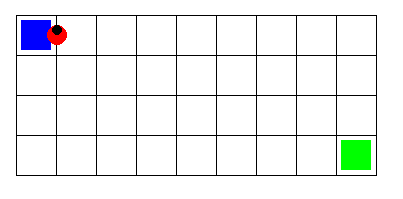
\includegraphics[width = \textwidth]{images/map2_easy.png}
    \caption{4x9 Gym Sapientino map for the experiment with two colors. The initial position is in the cell [2,4] in the center of the map.}
    \label{fig:mapTwoColors}
\end{figure}

\noindent
We present two progressive trials for this specific case, in particular in the second trial reaches properly the convergence. 

\begin{table}[h]
\begin{tabular}{|p{1cm} |p{2cm}||p{1cm}|p{1.5cm}|p{2cm}|p{1cm}|p{1cm}|p{1cm}|p{1.1cm}|  }
 \hline
 \multicolumn{9}{|c|}{Agent parameters} \\
 \hline
Trial & Algorithm name & batch size & memory & exploration & lr & update frequency &reward shaping & episodes \\
 \hline
trial1& PPO & 32 & 20000 & 0.4 & 0.001 & 32 & no & 2000 \\
\hline
\hline
trial2& PPO & 64 & 64 & 0.0 & 0.001 & 20&  yes &1000 \\
\hline
\end{tabular}
\caption{Table containing the relevant hyperparameter configuration of the tested agents related to the two experiments with two colors}
\end{table}

\noindent\\ \\
\textbf{Plots related to the first trial:}\\
%\includegraphics[scale=0.65]{images/reward1.png}\\
\includegraphics[scale=0.55]{images/episode_length1.png}
\includegraphics[scale=0.55]{images/episode_return1.png}



\noindent\\ \\
\textbf{Plots related to the second trial:}\\\\
%\includegraphics[scale=0.65]{images/reward_2.png}\\
\includegraphics[scale=0.55]{images/episode_length_2.png}
\includegraphics[scale=0.55]{images/episode_return_2.png}

\noindent
We can perform a comparison observing these following plots.
In particular, observing the plots related to the \textit{episode-length}, we can notice that in the second case the length of the episodes is quite reduced, this means that the agent reaches the temporal in a better manner and more frequently during the whole training phase.\\
Observing the \textit{episode-return} plots, we can notice that while in the first case the reward are always positive but quite sparse, in the second case (thanks to the reward shaping technique, that prods the agent to learn better) the rewards accumulated among the episodes tend to  stabilize around the same intervals of value. This means that in the second case the reward shaping represents a very important element in order to achieve the convergence. 


\noindent

\section{Experiments with two colors with  bigger maps}
In these experiments we have tried to train the agent with  big complex maps in order to the reach the temporal goal \textit{blue,green}.

\subsection{First Trial}

\begin{figure}[h]
    \centering
    \includegraphics[scale=0.70]{images/mappa_media.png}
    \caption{7x10 Gym-Sapientino map. The initial position is in cell [4,6] more or less in the center of the map.}
    \label{fig:twoColorIntermediateSizeMap}
\end{figure}


\noindent
\textbf{Plots related to this trial:}\\\\

\includegraphics[scale=0.55]{images/episode_len_media.png}
\includegraphics[scale=0.55]{images/episode_return_media.png}


\begin{table}[ht]
\begin{tabular}{|p{1cm} |p{2cm}||p{1cm}|p{1.5cm}|p{2cm}|p{1cm}|p{1cm}|p{1cm}|p{1.1cm}|  }
 \hline
 \multicolumn{9}{|c|}{Agent parameters} \\
 \hline
Trial & Algorithm name & batch size & memory & exploration & lr & update frequency &reward shaping & episodes \\

\hline
trial1& PPO & 64 & 64 & 0.25 & 0.001 & 20&  yes &1000 \\
\hline
\end{tabular}
\caption{Table containing the relevant hyperparameter configuration of the tested agents related to the  experiment with two colors in the first bigger map}
\end{table}

\noindent\\
In this case the agent has a good behaviour, slightly worse than in the previous case with a smaller map. The agent reaches the temporal goal quite frequently and thanks to the exploration parameter (set to 0.25) it can probe better the action space. Moreover observing also the \textit{episode-length} plot, we can observe that the length of the episodes is higher w.r.t. the previous trials with the small map.

\subsection{Second Trial}
\begin{figure}[h]
    \centering
    \includegraphics[scale=0.25]{images/bigmap.png}
    \caption{9x17 Gym-Sapientino map. The initial position is in cell [4,8] in the center of the map. }
    \label{fig:bigmap}
\end{figure}


\noindent\\ \\
\textbf{Plots related to this trial:}\\

\includegraphics[scale=0.55]{images/episode_len_map.png}
\includegraphics[scale=0.55]{images/episode_return_map.png}

\noindent\\
The rewards accumulated during the episodes are decidedly lower with respect to the previous experiments. In fact in this case the agent doesn't reach the goal frequently, the map is very large and despite the exploration addition, the agent's behaviour is decidedly worse.
Moreover, observing also the \textit{episode-length} plot, the episodes are decidedly longer than in the previous trials, and this means that almost always during the training phase the whole episode is executed, with all timesteps without  reaching the temporal goal.

\begin{table}[h]
\begin{tabular}{|p{1cm} |p{2cm}||p{1cm}|p{1.5cm}|p{2cm}|p{1cm}|p{1cm}|p{1cm}|p{1.1cm}|  }
 \hline
 \multicolumn{9}{|c|}{Agent parameters} \\
 \hline
Trial & Algorithm name & batch size & memory & exploration & lr & update frequency &reward shaping & episodes \\

\hline
trial1& PPO & 64 & 64 & 0.3 & 0.001 & 20&  yes &1000 \\
\hline
\end{tabular}
\caption{Table containing the relevant hyperparameter configuration of the tested agents related to the  experiment with two colors in the second bigger map}
\end{table}


\section{Experiment with three colors}

To increase task complexity and show how the agent reacts when an additional color is introduced in the goal sequence, we have tested maps with three colors. 
We experimented with the goal sequence  G = \{\color{blue} blue \color{black}, \color{red} red \color{black},\color{green} green \color{black}\} on a small 4X9 grid map without walls (figure[\ref{fig:mapThreeColors}]) and compared the results obtained by the baseline Tensorforce implementation with the implementation described in figure [\ref{fig:nonMarkovianNetwork}]. \\

The baseline network configuration is automatically configured based on input types and shapes, and it is characterized by: a \textit{retrieve layer}(input layer) that takes as input the state, two dense layers of size 64, one Register layer, an other Retrieve layer that takes as input the encoded state, two new dense layers of size 64, an other Register layer. Finally a Retrieve layer that concatenate the state and the encoded state tensors and a last dense layer of size 64.\\

We trained each of the two agents for 1000 episodes of with 300 maximum number of time steps each to create a common scenario for performance comparison. \\


Each experiment is performed using the reward shaping described in the section [\ref{sec:rewardShaping}] for three color goals.\\
Refer to the table [\ref{tab:threeColorMapAgentTable}] for description of the agent hyperparameter values.\\



\begin{figure}[ht]
  \centering
  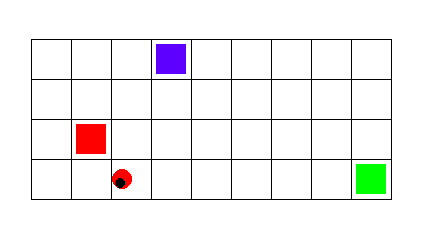
\includegraphics[width=\textwidth]{images/map3_easy.png}
\caption{4x9 Gym Sapientino map for the experiment with three colors. The initial position is in cell [4,4] at the bottom of the map.}
\label{fig:mapThreeColors}
\end{figure}

These two experiments have a dual objective:
\begin{itemize}
    \item First of all we motivated our choices in the proposed neural network implementation. In fact, with a baseline Tensorforce policy network which does not perform the separation between the color expert as shown in figure [\ref{fig:baselineSchema}] we cannot are not able to visit even a single color of the goal sequence, as shown in the \textit{episode-return} plot in figure [\ref{fig:threeColorsPlotsAuto}] where the reward is always negative, and thus we do not reach convergence  [\ref{fig:threeColorsPlotsAuto}].
    \item We have shown that our non markovian network is not limited in solving tasks with two colors only and proved that, using the same kind of approach that we used for two colors goals and simply extending the hidden layers to include an additional color expert, we are able to generalize on three colors as shown in the plots [\ref{fig:threeColorsPlotsCustom}].
\end{itemize}

We see that our proposed implementation agent reaches convergence in almost 800 episodes, after which, the goal is reached in more than 95\% of the episodes. Also the episode length stabilized after a while, showing that the agent has learnt a series of trajectory that bring it to the goal in 200 time steps on average (left plot in figure [\ref{fig:threeColorsPlotsCustom}]) , a time way shorter than the maximum time available in the experiment. This means not only that the agent has achieved the ability to visit the goal sequence in the correct order but also that it has learnt to do it "quickly"

\footnote{We also attached a video clip inside the video folder \textit{/video/three\textunderscore colors.mp4} which shows the described agent behaviour.}
which is often appreciable. \\







\begin{figure}[H]
  \centering
  \begin{minipage}[b]{0.45\textwidth}
    \includegraphics[width=1.2\textwidth]{images/episode_length3.png}
  \end{minipage}
  \hfill
  \begin{minipage}[b]{0.45\textwidth}
    \includegraphics[width=1.2\textwidth]{images/episode_return3.png}
  \end{minipage}
  \caption{Plots related to the first trial with three colors and with our custom network.}
  \label{fig:threeColorsPlotsCustom}
\end{figure}


\begin{figure}[H]
  \centering
  \begin{minipage}[b]{0.45\textwidth}
    \includegraphics[width=1.2\textwidth]{episode_length_auto.png}
  \end{minipage}
  \hfill
  \begin{minipage}[b]{0.45\textwidth}
    \includegraphics[width=1.2\textwidth]{episode_return_auto.png}
  \end{minipage}
  \caption{Plots related to the first trial with three colors and with auto network.}
  \label{fig:threeColorsPlotsAuto}
\end{figure}





\begin{table}[h]
\begin{tabular}{|p{2.3cm} |p{1.8cm}|p{1.5cm}|p{1.5cm}|p{1.cm}|p{0.6cm}|p{1cm}|p{1.1cm}| p{1.1cm}|  }
 \hline
 \multicolumn{9}{|c|}{Agent parameters for the three color goal experiments in the 4X9 map.} \\
 \hline
 Agent name & batch size & memory & hidden size & expl. & lr & update freq. &rew. shap. & episodes \\
 \hline
 PPO baseline & 64 & 64 & 64 & 0.0 & $10^{-3}$ & 20 & yes & 2000  \\
\hline
\hline
 Our approach & 64 & 64 & 192 & 0.0 & $10^{-3}$ & 20&  yes &1000 \\
\hline
\end{tabular}
\caption{Table containing the relevant hyperparameter configuration of the tested agents on the three color map. The proposed implementation features 193 neurons on the two hidden layers. This happens since in order to reach the temporal goal we need 3 experts. Using 64 neurons for each expert we have \(193 = 64*3\) hidden neurons.}
\label{tab:threeColorMapAgentTable}
\end{table}






\section{Conclusion and result discussion}
%Parte aggiunta dopo. Controllare in seguito.
In this paper we have proposed a Tensorforce based non markovian agent implementation which is able to solve a non markovian navigation task in the Gym-Sapientino two dimensional map.
We proved the effectiveness of the presented approach by showing that our agent converges when solving the tasks with two color goal formulas and that we can easily generalize on three colors by simply extending the hidden layers to include the additional color expert. \\
We discussed the benefits of reward shaping and proved that the sparse reward problem, which was one of the major issue our agent experienced in the training process, can be easily overcome by introducing intermediate positive rewards which boost the learning process and, in our opinion, encourages the agent to complete the various steps that are needed to reach the goal.\\
However, even using reward shaping, we found out that reward sparsity can still be experienced on larger maps (figure [\ref{fig:twoColorIntermediateSizeMap}],[\ref{fig:bigmap}]). This happens since the state space becomes much larger and, we reckon, it is very likely that the agent get stuck in exploring \textit{"white"} regions of the map not learning any useful trajectory and receiving constant negative rewards. If it is the case, it may happen that the agent converges sub-optimally which results in a policy that leads to always negative reward action selection. In fact, since PPO updates are based on direct experience and do not use any experience replay buffer by default, we are persuaded that in order to learn a successful policy that allows to frequently visit the goal sequence, the agent should sample the goal as much as possible. \\
For this purpose, we proved also the benefits of including some exploration in order to force the agent to probe the action space more effectively.\\
We have also uploaded the related code into a \href{https://github.com/francycar/RA_project}{github repository}.



\footnote{Exploring the action space often leads to the  execution of sub-optimal actions. However, if the agent is already behaving sub-optimally, an exploration phase may lead the agent to discover new trajectories that lead to higher rewards on the long run.} .\\













\bibliography{main}
\bibliographystyle{plain}

\begin{itemize}
   \bibitem{Gym-Sapientino}
\url{https://github.com/cipollone/gym-sapientino-case/tree/master/gym\_sapientino\_case}{}

\end{itemize}



























\end{document}
